\section{Distributed K Nearest Neighbor}

\vspace{5 mm}
\noindent
We would like to use a spill tree model on our data to categorize data with 
some likelihood of being close to our chosen data point. Once we 
construct the spill tree, classifying a point would then be as simple as 
performing a look up for the point (which would have complexity $O(P D)$ where 
$D = $ the depth of the spill tree) and then computing K Nearest Neighbor on 
the subset of the data, which if we set a threshold of the size of our child 
node equal to $U$ would be $O(U^{2} P)$ for a total time complexity of 
$O(P D + C^{2} P)$. Compared to our naive way of doing K Nearest Neighbor, 
this classification scheme with $U << N$, our runtime on classification is much 
less.

\vspace{5 mm}
\noindent
However, there are numerous problems when implementing a spill tree directly 
on our whole data set.

\begin{itemize}
\item Constructing our $D$ matrix in our spill tree algorithm is already  
$O(N^{2} p)$, so implementing a spill tree may help us for lookup, but will not 
help us in avoiding the time complexity of actually making the spill tree.
\item For data size large enough that it will not fit on a single machine, 
calculating a spill tree directly in a distributed environment will be 
near-impossible. Like K Nearest Neighbor, to construct a spill tree with 
perfect precision, we need to compare each data point to every other data 
point to determine the furthest two data points. On a distributed setting, this 
is impossible without a lot of computer communication.
\end{itemize}

\vspace{5 mm}
\noindent
Instead of constructing a spill tree on all of our data, we will instead 
implement an approximate hybrid spill tree. This approximation method will 
construct a sampled hybrid spill tree on one machine. This spill tree will 
classify our data into chunks of data that can fit on single machines. From 
there, we construct a spill tree on each of the distributed data sets.

\vspace{5 mm}
\noindent
The main problem with using a normal spill tree as our data structure is that is
$\tau$ is too large, the depth of the spill tree can go to infinity.  To prevent
this, we can use a hybrid spill tree.  Hybrid spill trees operate identically to
spill trees, except they have an additional parameter $\rho$, with $0 \le \rho <
1$  such that if the overlap proportion when $P.lc$ and $P.rc$ are constructed
is  $> \rho$, then $P.lc$ and $P.rc$ are instead simply split on the initial
bound  $B$, with no overlap.  These nodes are marked as non-overlap, which will
become  important later on.  This guarantees that we will not have an infinite
depth  tree, and makes spill trees usable for our application.

\vspace{5 mm}
\noindent
We will be using a hybrid spill tree to store our data, because it will allow us
to make efficient approximate K nearest neighbor searches.  On a standard spill
tree with overlaps we would use defeatist search to implement K nearest
neighbors,  but it is important to remember that we now have non-overlap nodes
scattered  throughout, for which we would instead use the standard metric tree
depth first search.

\vspace{5 mm}
\noindent
This gives us an efficient data structure to use for our K nearest neighbors
algorithm, but it is still designed to be used in a serial environment, and we
want to use this in a distributed environment.  To accomplish this we will have
to somehow split the dataset among multiple machines.  This is problematic, as
to generate a hybrid spill tree, you need to have all of the data accessible in
memory.  We solve this by using the following procedure:

\hrulefill
\begin{figure}[h]
\centering
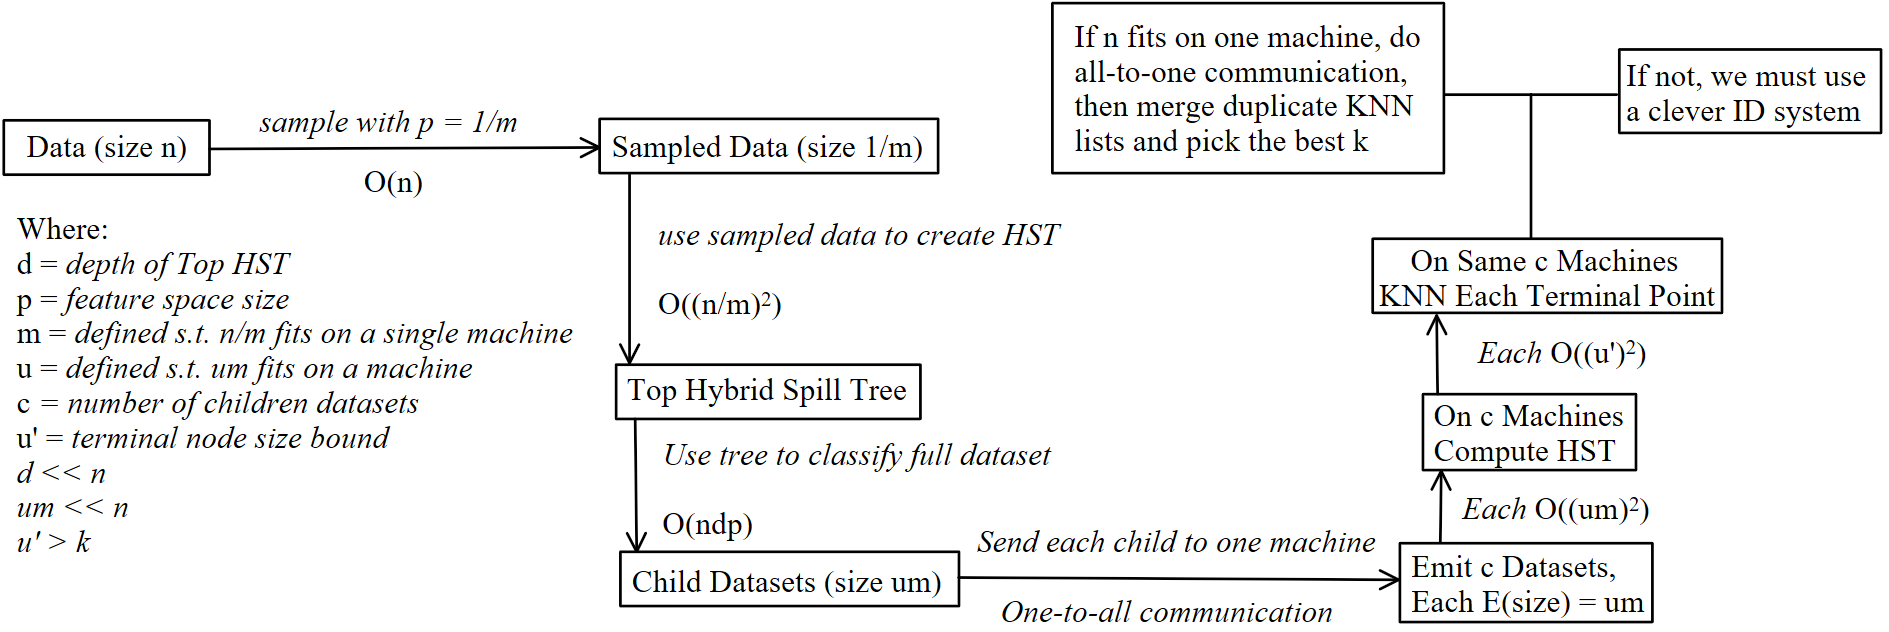
\includegraphics[width=0.9\textwidth]{algorithm}
\caption{A visualization of our algorithm to solve distributed K Nearest Neighbors}
\end{figure}
\hrulefill

\vspace{5 mm}
\noindent
\textbf{ADD QUICK EXPLANATION OF WHAT IS GOING ON HERE} 

\vspace{5 mm}
\noindent
This procedure works because the hybrid spill trees yield children subsets that,
with high probability, contain nodes that are close together.  This is true for 
hybrid spill trees more so than metric trees because in a metric tree, two points
that are very close together can be split into two different subtrees and never be
compared, but this does not happen in a hybrid spill tree.  In our algorithm, even
if two similar points happen to be separated in one of the children resulting from
a split, they will still be together in the other child, and so during evaluation 
it will still be considered.  This property can be seen below:

\vspace{5 mm}
\noindent
\hrulefill
\begin{figure}[h]
\centering
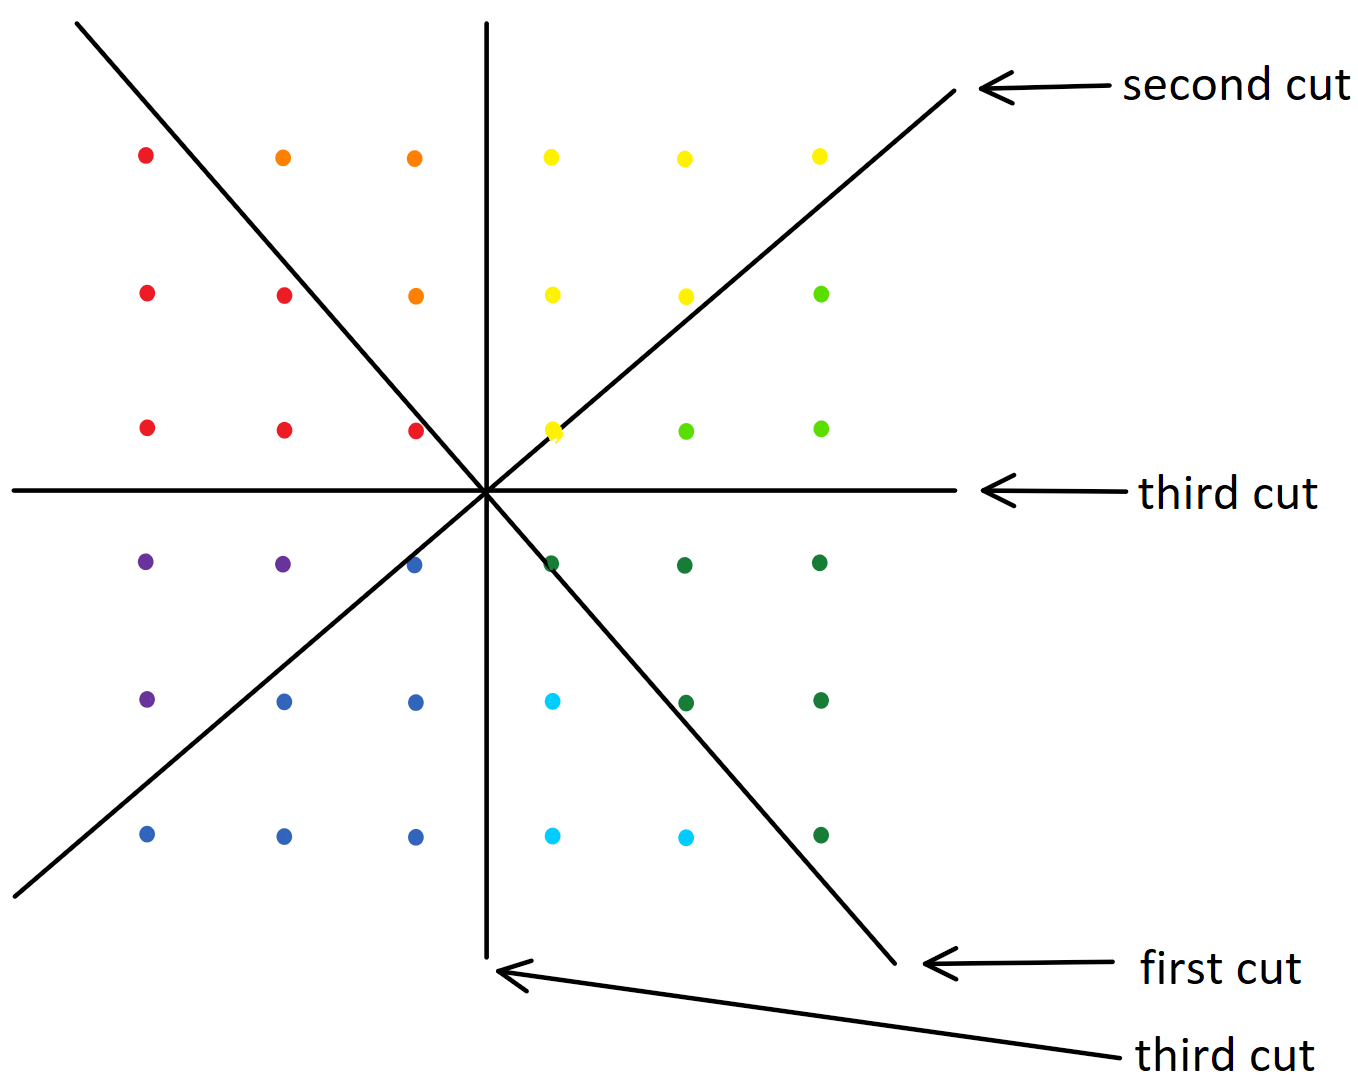
\includegraphics[width=0.9\textwidth]{metric}
\caption{In the metric tree, two points that are very close together will not 
be evaluated, whereas two points much further apart will be, because they 
happen to be in the same split}
\end{figure}
\hrulefill

\vspace{5 mm}
\noindent
\hrulefill
\begin{figure}[h]
\centering
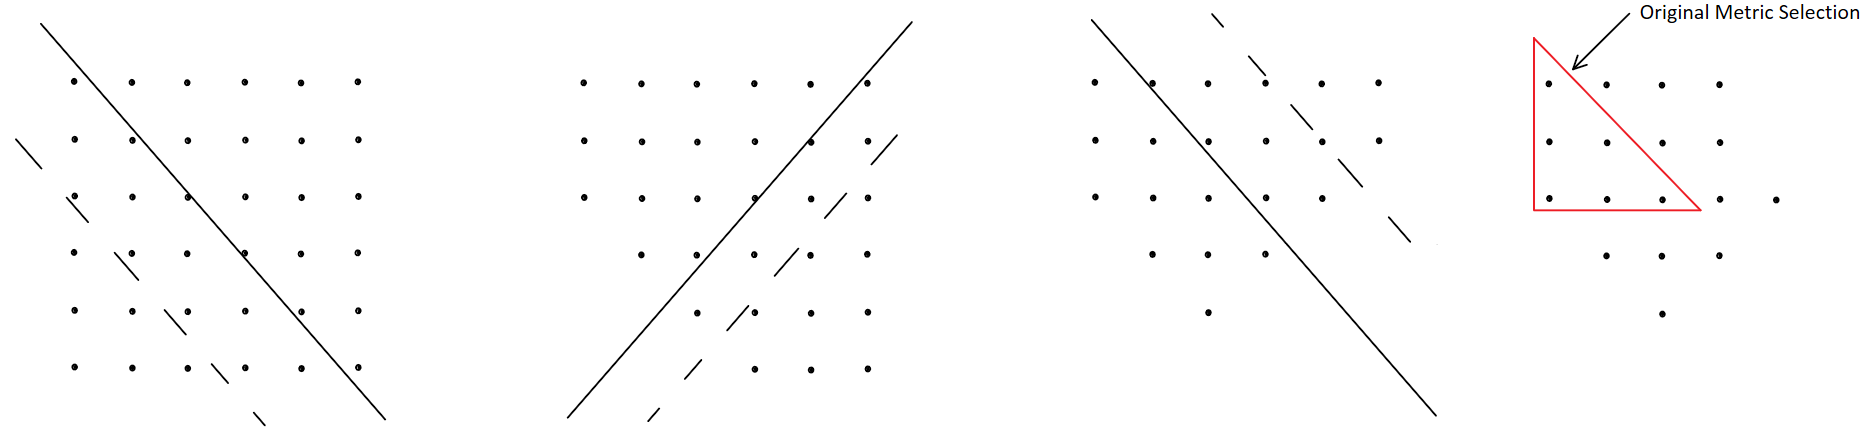
\includegraphics[width=0.9\textwidth]{spill}
\caption{In the spill tree, we can see that when comparing the corresponding
subset, there are much better odds of close together points being evaluated
together}
\end{figure}
\hrulefill

\vspace{5 mm}
\noindent
\textbf{TALK ABOUT COMM COSTS AND SUCH}

\vspace{5 mm}
\noindent
One of the advantages to our algorithm is that the runtime is heavily 
modifiable.  Some of our user parameters such as $m$ and $u$ are tuned according
to memory constraints or dataset size, but we can adjust $\tau$ and $\rho$ to 
bring down the runtime of our algorithm at the expense of accuracy, or increase 
the accuracy at the expense of the runtime.  Once you fit an initial model it is 
convenient to be able to optimize your accuracy, subject to your personal time 
constraints.  Consider our top tree, we know that when $\tau$ is 0 the model 
becomes metric, and that as $\tau$ increases the overlap will become greater and 
greater between pairs of children nodes.  It is therefore important to keep 
$\tau$ relatively low in the top tree, where a large amount of overlap will 
result in a greater compute time in the tope tree, as well as many more 
computations down the line when we are using our bottom trees.  In the bottom 
trees, however, it is less important to keep $\tau$ low, as multiple machines 
are making their spill tree computations in parallel, and we can afford to allow 
more overlap, as long as we set an appropriate value for $\rho$ to prevent the 
tree depth from getting out of hand.  Overall, the user defined parameters give 
our model a large degree of customization, and allow it to become optimized for 
the problem at hand.
